\documentclass[10pt,conference]{IEEEtran}
\usepackage[T1]{fontenc}
\usepackage{graphicx,booktabs,amsmath,amssymb,cite,xcolor,url,microtype}
\newcommand{\pending}[1]{\textcolor{red}{\textbf{[PENDING: #1]}}}
\renewcommand{\arraystretch}{1.08}
\begin{document}
\title{Post-hoc Quantization of Local Feature Descriptors:\\ What Matters at Which Bit-width?}
\author{\IEEEauthorblockN{Donghyun Lim}
\IEEEauthorblockA{Department of Computer Science, SUNY Korea\\ CSE 527 Course Project Report, Fall 2026}}
\maketitle

\begin{abstract}
Learned local descriptors are stored as floating-point vectors, which makes large maps expensive to store. We study how far a descriptor can be compressed \emph{after} the network is trained, using only a small calibration set and no retraining. With XFeat (64-D, 256 bytes) frozen, we compare, under one protocol, scalar quantization (six calibration strategies, five bit-widths, three distances), dimensionality reduction (PCA and Gram--Schmidt Feature Reduction), product quantization, and thresholds and projections learned with a differentiable thermometer code. Three results stand out. At 4 bits per dimension (32 bytes, $8\times$ smaller) every training-free family stays within about 0.7 points of float precision. Below that budget, accuracy depends on the calibration rule and on whether correlation between dimensions is used, and the best choice differs between XFeat and SIFT. Learned thresholds do not improve on quantile calibration, and a learned projection wins on the training distribution but loses on HPatches. Against an equally optimized float matcher, compact codes are only 1.0--2.1$\times$ faster, so the clear benefit is memory. All numbers are validation results; a pre-registered held-out evaluation is specified.
\end{abstract}
\begin{IEEEkeywords}
Local features, descriptor compression, quantization, calibration, image matching.
\end{IEEEkeywords}

\section{Introduction}
Local feature matching underlies SLAM, structure-from-motion and visual localization. As maps grow, descriptor storage becomes a bottleneck: even a lightweight extractor such as XFeat~\cite{xfeat} outputs 64 floats (256 bytes) per keypoint. Existing remedies fall into three groups. Learned compression, e.g.\ Differentiable Product Quantization (DPQ)~\cite{dpq}, trains a scene-specific auto-encoder. Dimensionality reduction, e.g.\ PCA or Gram--Schmidt Feature Reduction (GFR)~\cite{gfr}, lowers the number of dimensions but keeps floats. Scalar quantization, the standard tool for neural-network inference~\cite{nagel,gholami}, lowers the bits per dimension. These families are rarely compared at the same number of bytes, with the same data and the same matcher.

This report is such a comparison. We do not propose a new method. We ask four questions: (i) which design choice matters at which bit-width; (ii) at equal bytes, is it better to cut bits, cut dimensions, or use vector quantization; (iii) does learning the quantizer beat calibrating it; and (iv) do the conclusions carry over to another descriptor.

Our contributions are: a 90-configuration study of calibration, bit-width and distance for XFeat with a decomposition of where accuracy is lost; an equal-byte comparison of scalar quantization, PCA/GFR and product quantization; a differentiable thermometer code (a relaxed XOR) used to learn thresholds and projections, with an analysis of when learning fails; and memory/speed measurements against a fair float baseline, a repetition on SIFT~\cite{sift}, and a pre-registered protocol for a held-out test.

\section{Related Work}
\subsection{Descriptor Compression}
Binary descriptors such as BRIEF~\cite{brief} and ORB~\cite{orb} are compact by construction but are not obtained from a learned float descriptor. Product quantization (PQ)~\cite{pq} splits a vector into sub-vectors and stores one codebook index per sub-vector; OPQ~\cite{opq} adds a rotation. DPQ~\cite{dpq} targets visual localization with SuperPoint map descriptors. The PQ codebooks, initialized by k-means, are made trainable through a soft assignment with a straight-through estimator, and a scene-specific two-layer MLP decodes the stored codes back to float descriptors before matching. Training needs only the descriptors of the scene's own map, with triplet margin losses and hard negatives in the original and decoded spaces; in their ablation the triplet loss, rather than L2 reconstruction, accounts for most of the gain on night-time queries. Queries are kept in float, and plain PQ is reported to be a strong baseline at moderate budgets. GFR~\cite{gfr}, built on the function-space Gram--Schmidt procedure of~\cite{gfrorig}, is a sequential PCA deflation that also removes degree-2 polynomial dependence; its authors report gains over PCA on SIFT and smaller gains on the learned HardNet descriptor~\cite{hardnet}. Both DPQ and GFR exploit relations between dimensions, which per-dimension scalar quantization ignores.

\subsection{Quantization Calibration in Neural Networks}
Post-training quantization chooses a clipping range from a few calibration batches~\cite{nagel,gholami}. Min--max covers the full range but is sensitive to outliers; percentile clipping and MSE-optimal ranges trade clipping error against rounding error~\cite{jacob,nagel}; non-uniform quantizers place levels by Lloyd--Max~\cite{lloyd}. Nagel \emph{et al.}~\cite{nagel} report that range setting matters little at 8 bits and much more at low bit-widths, and that MSE is a poor criterion when only the order of values matters. Descriptor matching is such a case: what must be preserved is the nearest-neighbour ranking. Because rounding has zero gradient, quantization-aware training uses the straight-through estimator (STE)~\cite{ste}, and methods such as LSQ~\cite{lsq} learn the step size. We apply these ideas to descriptors and test which of the conclusions survive.

\section{Method}
\subsection{Pipeline and Scalar Quantization}
XFeat is frozen. Its descriptor $x\in\mathbb{R}^{64}$ is $\ell_2$-normalized. For each dimension $d$ a set of $L-1$ ordered thresholds $t_{d,1}<\dots<t_{d,L-1}$ is computed once from calibration descriptors, and the code is
\begin{equation}
c_d(x)=\sum_{k=1}^{L-1}\mathbf{1}[x_d>t_{d,k}]\in\{0,\dots,L-1\}.
\end{equation}
We compare six ways of setting the thresholds, each a standard choice in network quantization: \emph{uniform} (per-dimension min--max, equal width), \emph{percentile} (0.1--99.9\% clip, equal width), \emph{quantile} (equal frequency), \emph{Lloyd--Max} (MSE-optimal, non-uniform), and \emph{shared} uniform and quantile variants that use one set of thresholds for all dimensions (per-tensor instead of per-channel). We use $L\in\{4,8,16,32,256\}$, i.e.\ 2--8 bits per dimension and 16--64 bytes per descriptor. An int8 per-tensor quantizer with an integer dot product serves as the conventional baseline.

\subsection{Distances}
Three distances are computed on the same codes: \emph{index-L1} $\sum_d|c_d-c'_d|$, \emph{index-L2} $\sum_d(c_d-c'_d)^2$, and \emph{reconstruction cosine}, the cosine between vectors in which each code is replaced by the calibration mean of its bin. If codes are stored as thermometer bits $b_{d,k}=\mathbf{1}[x_d>t_{d,k}]$, index-L1 equals the Hamming distance and is computed with XOR and popcount; this was the starting point of the project (8 levels, 56 bytes).

\subsection{Other Training-free Families}
\emph{PCA/GFR + scalar}: descriptors are projected to $m$ dimensions and each coordinate is quantized as above ($m\cdot\log_2 L/8$ bytes). GFR is our re-implementation of Algorithm~2 of~\cite{gfr} with degree-2 multilinear terms; with degree-1 terms only it reproduces the PCA subspace to $10^{-13}$. \emph{PQ}: $M$ sub-vectors with $K{=}256$ k-means centroids each ($M$ bytes), with or without a PCA rotation whose dimensions are interleaved across sub-vectors. All projections and codebooks are fitted on the calibration descriptors only.

\subsection{Differentiable Thermometer Code}
XOR is not differentiable. We relax a thermometer bit to $s_{d,k}=\sigma((x_d-t_{d,k})/\tau)$ and the XOR of two bits $p,q$ to
\begin{equation}
p\oplus q\;\approx\;p(1-q)+(1-p)q ,
\end{equation}
which equals the Hamming distance when $p,q\in\{0,1\}$. With the straight-through estimator~\cite{ste}, the device DPQ uses for its soft centroid assignment~\cite{dpq}, the forward pass uses hard bits and the backward pass the gradient of $s$, so the training distance is exactly the test-time distance. Thresholds, and optionally a projection matrix initialized with PCA, are trained with a symmetric cross-entropy over the distance matrix of an image pair, using ground-truth correspondences given by the homography.

\section{Experiments}
\subsection{Setup}
\textbf{Calibration.} 191,581 XFeat descriptors from 192 COCO val2017 images~\cite{coco} (longest side 640, 1000 keypoints). \textbf{Training/development} (learning experiments only): 600/192 synthetic-homography pairs from 200/64 further COCO images. \textbf{Validation.} 192 synthetic pairs from 64 other COCO images, and all 580 pairs (image 1 vs.\ 2--6) of HPatches~\cite{hpatches}. No image is shared between these sets. Validation data were used to compare configurations and are therefore not called a test set. \textbf{Metric.} Mutual nearest-neighbour matches (ties to the smallest index); a match is correct if its reprojection error is below 3 px; we report pooled precision (correct/mutual, \%), as ``HPatches / COCO''. Float XFeat reaches 60.59 / 70.57.

\begin{figure*}[t]
\centering
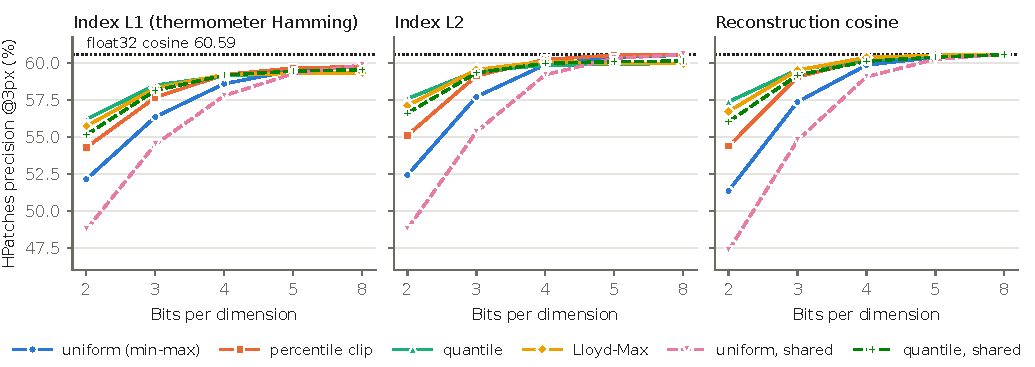
\includegraphics[width=0.96\textwidth]{fig2.pdf}
\caption{XFeat on HPatches (validation): precision at 3\,px for six calibration strategies, five bit-widths and three distances. Dashed lines use thresholds shared by all dimensions. The dotted line is the float descriptor.}
\label{fig:matrix}
\end{figure*}

\subsection{What Matters at Which Bit-width}
Fig.~\ref{fig:matrix} shows the 90 configurations. At 2 bits the calibration rule dominates: quantile reaches 57.59 with index-L2 while uniform reaches 52.42 and shared uniform 48.77. From 5 bits on, the strategies are within about 0.6 points for a given distance, and the distance decides the order: index-L1 saturates near 59.8, whereas index-L2 and reconstruction cosine reach 60.5--60.6. With index-L2 at high bit-widths, uniform and percentile thresholds are about 0.5 points better than quantile, the reverse of the 2-bit order. This matches the observation for network activations that range setting matters most at low bit-widths~\cite{nagel}. The int8 baseline gives 60.58 / 70.54, i.e.\ no loss.

For the original 8-level thermometer code (58.51), replacing index-L1 by reconstruction cosine on the same codes recovers 1.05 of the 2.08 lost points, so on HPatches half of the loss is due to the distance and half to quantization. The split is not universal: it is 26:74 (quantization:distance) with 16 levels on HPatches and 74:26 with 8 levels on COCO.

\subsection{Memory and Speed}
\begin{table}[t]
\caption{Memory and matching speed for XFeat. Speed-ups are relative to the fastest float matcher (one BLAS GEMM). Two-image: 1000$\times$1000 mutual matching including encoding. 1-NN: exact search in 65k--524k descriptors (range over three sizes and two runs).}
\label{tab:speed}
\centering\footnotesize
\begin{tabular}{@{}lrrrr@{}}
\toprule
Representation & Bytes & HPatches & Two-image & 1-NN\\
\midrule
float32, cosine & 256 & 60.59 & 1.00$\times$ & 1.00$\times$\\
int8, dot & 64 & 60.58 & 1.13$\times$ & 1.31--1.52$\times$\\
8 levels, index-L2 & 64 & 59.46 & 1.35$\times$ & 1.64--1.91$\times$\\
8 levels, index-L1 & 64 & 58.51 & 1.48$\times$ & 1.67--2.06$\times$\\
8 levels, thermometer & 56 & 58.51 & 1.25$\times$ & 1.03--1.26$\times$\\
16 levels, packed, L2 & 32 & 60.25 & --- & 1.36--1.54$\times$\\
\bottomrule
\end{tabular}
\end{table}
Table~\ref{tab:speed} lists storage and speed (AVX2, two threads; extraction time excluded). Storage shrinks by 4--8$\times$ at a cost of about 2 points or less. Speed gains are modest: 1.1--1.5$\times$ for matching two images and 1.0--2.1$\times$ for large-scale search, and they do not grow with database size. An earlier figure of 3.75$\times$ for the thermometer code was measured against XFeat's reference matcher, which computes the similarity matrix twice; against a single-GEMM float matcher the same code is 1.25$\times$ faster. Float inner products are already well optimized, so the benefit of compression is memory and transmission size. Timings for the packed 4-bit code in the two-image setting and for the families of Section~\ref{sec:families} were not measured.

\subsection{Equal-byte Comparison of Families}\label{sec:families}
\begin{table}[t]
\caption{Precision at 3\,px (HPatches / COCO) at equal bytes, XFeat. Scalar: 64-D with quantile (2, 3 bit) or percentile (4 bit) thresholds, index-L2. PCA+scalar: 32-D$\times$2 bit, 32-D$\times$4 bit, 48-D$\times$4 bit, 32-D$\times$8 bit. PQ: PCA rotation, $M$ = bytes, $K$ = 256. Learned: projection and thresholds trained on synthetic COCO pairs (16-D, 32-D, 48-D, 64-D at 4 bit). Float: 60.59 / 70.57.}
\label{tab:families}
\centering\footnotesize
\setlength{\tabcolsep}{3.5pt}
\begin{tabular}{@{}rcccc@{}}
\toprule
Bytes & Scalar 64-D & PCA + scalar & PQ & Learned proj.\\
\midrule
8 & --- & 53.73 / 64.47 & 52.64 / 60.79 & 53.25 / 68.94\\
16 & 57.59 / 66.84 & 59.10 / 69.54 & 59.31 / 68.94 & 58.01 / 70.44\\
24 & 59.46 / 69.34 & 59.97 / 70.05 & --- & 58.43 / 70.50\\
32 & 60.25 / 70.05 & 59.90 / 70.52 & 60.45 / 70.46 & 58.13 / 70.53\\
\bottomrule
\end{tabular}
\end{table}
Table~\ref{tab:families} compares the families at the same storage. At 32 bytes the three training-free families are within about 0.6 points of each other and 0.7 of float. At 16 bytes the methods that use correlation between dimensions are ahead: PCA to 32-D with 4 bits and PCA-rotated PQ both gain 1.5--1.7 points on HPatches (2.1--2.7 on COCO) over 2-bit scalar quantization. PQ without the rotation gives 57.20 / 65.40, no better than 2-bit scalar codes, so the gain comes from the rotation, not from vector quantization as such. At 8 bytes all training-free methods lose 6 points or more.

Dimensionality reduction alone is not competitive: 32-D float PCA (128 bytes) gives 59.91 / 70.51, below 4-bit scalar codes of a quarter the size. XFeat nevertheless has redundancy: 48 PCA dimensions keep 99.3\% of the variance and match 64-D float accuracy. GFR and PCA are indistinguishable on XFeat: over 68 matched configurations the mean difference is 0.01 points on HPatches and 0.07 on COCO, consistent with the small gains reported in~\cite{gfr} for a learned descriptor. If only the database is compressed and queries stay in float, the setting used by DPQ~\cite{dpq}, the loss shrinks: at 16 bytes the three families reach 59.0, 59.5 and 60.0 on HPatches.

\subsection{Does Learning Beat Calibration?}
\textbf{Thresholds.} Training the thresholds of 64-D codes from quantile initialization changes validation precision by less than 0.3 points in every setting (2 bit, index-L2: 57.59 $\rightarrow$ 57.51 on HPatches, 66.84 $\rightarrow$ 66.86 on COCO; the relaxed-XOR loss behaves the same). The optimizer itself works: started from uniform thresholds it recovers from 52.42 to 57.53, the quantile level. For per-dimension thresholds on XFeat, equal-frequency calibration is already near the optimum of the matching loss.

\textbf{Projection.} Training a projection jointly with the thresholds (last column of Table~\ref{tab:families}) gives the best COCO numbers at every budget, +4.5 points at 8 bytes, and on the development pairs a 16-byte code reaches 69.20 against 69.36 for float. On HPatches the same models are below the training-free methods by 1.1--1.3 points at 16 bytes and 2.1--2.3 at 32 bytes. The gap widens with the amount of training: at 16 bytes, thresholds-only training gives 58.94 / 69.72 and full training 58.01 / 70.44. The projection adapts to the synthetic-warp distribution it was trained on, whereas calibration-only compression keeps its ranking across both datasets.

\subsection{Generalization to SIFT}
\begin{table}[t]
\caption{Do the XFeat conclusions hold for SIFT (128-D)? HPatches precision at 3\,px. Spread: best minus worst of the six calibrations (index-L2 for XFeat, index-L1 for SIFT).}
\label{tab:sift}
\centering\footnotesize
\setlength{\tabcolsep}{3pt}
\begin{tabular}{@{}p{2.55cm}p{2.6cm}p{2.9cm}@{}}
\toprule
Question & XFeat & SIFT\\
\midrule
Loss at 8 bit & none (60.58 vs.\ 60.59) & none (61.08 vs.\ 61.07)\\
Spread between calibrations at 2 bit & 8.8 points & 7.2 points\\
Best calibration, 2 bit & quantile & Lloyd--Max, percentile (quantile is worst)\\
Distance order & L2 $\approx$ cosine $>$ L1 & L1 $>$ L2 $>$ cosine\\
Cut dimensions or bits (same bytes) & PCA + 4 bit (59.10 vs.\ 57.59) & 2 bit (63.65 vs.\ 61.41)\\
\bottomrule
\end{tabular}
\end{table}
We repeated the study with OpenCV SIFT~\cite{sift} on the same images and homographies (158,176 calibration descriptors). SIFT values are non-negative and skewed, with 17\% exact zeros. Table~\ref{tab:sift} summarizes the outcome. What transfers: 8 bits cost nothing, and calibration matters most at low bit-widths. What does not: quantile thresholds collapse onto repeated values and are the worst per-dimension choice at 2 bits; L1 is the better distance, also for float SIFT (66.2 vs.\ 62.3 with L2 on a quarter of the pairs), in line with the known benefit of non-Euclidean comparison for SIFT~\cite{rootsift}; and keeping all 128 dimensions at 2 bits beats PCA to 64-D at 4 bits.

Precision must be read with care here. The highest SIFT precision (67.55, Lloyd--Max, 2 bit, index-L1) comes with 11\% fewer mutual matches and 1.6\% fewer correct matches than float, while quantile at 2 bits has the lowest precision but 4\% more correct matches than float. For XFeat at 2 bits, precision and the number of correct matches rank the six calibrations identically.

\subsection{Held-out Evaluation}
MegaDepth-1500~\cite{megadepth,loftr} has not been used in this project. Fifteen configurations and ten directional predictions (e.g.\ ``at 16 bytes, PCA 32-D$\times$4 bit beats 64-D$\times$2 bit'') are fixed in a pre-registration file together with checksums of all thresholds, projections and codebooks; the list is run once and every outcome is reported. \pending{pose AUC@5/10/20 for the 15 configurations and the outcome of the ten predictions.}

\section{Discussion and Limitations}
\textbf{When to use what.} Scalar quantization needs no training, one calibration pass and only comparisons to encode, and its codes can be matched directly with integer arithmetic. For XFeat it is sufficient down to 4 bits per dimension. Below that, a PCA projection before quantization costs one matrix product per descriptor and recovers 1.5--2.7 points. PQ offers no accuracy advantage over PCA + scalar at 16--32 bytes in our tests. Learned compression can exceed all of them on data resembling its training set, but our projection learned on synthetic warps did not transfer to HPatches. DPQ avoids this gap by construction, since it is trained on the descriptors of the very map it compresses~\cite{dpq}, at the price of training per scene.

\textbf{Why thresholds are not the bottleneck.} Learning leaves quantile thresholds essentially unchanged, while a rotation helps. The loss at 2--3 bits is therefore a limit of treating dimensions independently, not of threshold placement.

\textbf{Limitations.} (i) All reported numbers are validation results on data that were also used to compare configurations; differences below about 0.5 points should not be read as rankings, and the held-out run is pending. (ii) DPQ was not reproduced, and GFR is our re-implementation, not the authors' code. (iii) The learning experiments use one loss, a linear map, one or two seeds and synthetic training pairs; more varied training data may transfer better. (iv) Speed was measured only for scalar codes with CPU brute-force matching; encoding cost and matching speed of PCA and PQ codes, GPUs and approximate indices were not measured. (v) Only XFeat and SIFT were tested; higher-dimensional learned descriptors such as SuperPoint~\cite{superpoint} were not. (vi) Precision alone can mislead when the number of matches changes, as the SIFT results show.

\section{Conclusion}
For compressing a frozen local descriptor, calibration was enough in our experiments and training was not needed. Up to $8\times$ compression, 4-bit scalar quantization matches float precision to within 0.3--0.5 points on validation data. For smaller codes the right choice depends on the descriptor's value distribution: for XFeat, reduce dimensions with PCA instead of going below 4 bits and use quantile thresholds; for SIFT, keep the dimensions, use Lloyd--Max or percentile thresholds and an L1 distance. A new descriptor should be checked with the same comparison before a rule is adopted. The main gain of compression is memory; matching speed improves by at most about $2\times$ over a well-implemented float matcher.

\begin{thebibliography}{99}
\footnotesize
\bibitem{xfeat} G. Potje, F. Cadar, A. Araujo, R. Martins, and E. R. Nascimento, ``XFeat: Accelerated features for lightweight image matching,'' in \emph{Proc. CVPR}, 2024.
\bibitem{dpq} Z. Laskar, I. Melekhov, A. Benbihi, S. Wang, and J. Kannala, ``Differentiable product quantization for memory efficient camera relocalization,'' in \emph{Proc. ECCV}, 2024.
\bibitem{gfr} K. Safavigerdini, B. Yaghooti, B. Sinopoli, and K. Palaniappan, ``Gram-Schmidt feature reduction for local feature descriptor compression,'' in \emph{Proc. CVPR Workshops}, 2026.
\bibitem{nagel} M. Nagel, M. Fournarakis, R. A. Amjad, Y. Bondarenko, M. van Baalen, and T. Blankevoort, ``A white paper on neural network quantization,'' arXiv:2106.08295, 2021.
\bibitem{gholami} A. Gholami, S. Kim, Z. Dong, Z. Yao, M. W. Mahoney, and K. Keutzer, ``A survey of quantization methods for efficient neural network inference,'' arXiv:2103.13630, 2021.
\bibitem{sift} D. G. Lowe, ``Distinctive image features from scale-invariant keypoints,'' \emph{Int. J. Comput. Vis.}, vol. 60, no. 2, pp. 91--110, 2004.
\bibitem{brief} M. Calonder, V. Lepetit, C. Strecha, and P. Fua, ``BRIEF: Binary robust independent elementary features,'' in \emph{Proc. ECCV}, 2010.
\bibitem{orb} E. Rublee, V. Rabaud, K. Konolige, and G. Bradski, ``ORB: An efficient alternative to SIFT or SURF,'' in \emph{Proc. ICCV}, 2011.
\bibitem{pq} H. J\'egou, M. Douze, and C. Schmid, ``Product quantization for nearest neighbor search,'' \emph{IEEE Trans. Pattern Anal. Mach. Intell.}, vol. 33, no. 1, pp. 117--128, 2011.
\bibitem{opq} T. Ge, K. He, Q. Ke, and J. Sun, ``Optimized product quantization for approximate nearest neighbor search,'' in \emph{Proc. CVPR}, 2013.
\bibitem{gfrorig} B. Yaghooti, N. Raviv, and B. Sinopoli, ``Gram-Schmidt methods for unsupervised feature extraction and selection,'' \emph{IEEE Trans. Inf. Theory}, vol. 71, no. 10, pp. 7856--7885, 2025.
\bibitem{hardnet} A. Mishchuk, D. Mishkin, F. Radenovi\'c, and J. Matas, ``Working hard to know your neighbor's margins: Local descriptor learning loss,'' in \emph{Proc. NeurIPS}, 2017.
\bibitem{jacob} B. Jacob \emph{et al.}, ``Quantization and training of neural networks for efficient integer-arithmetic-only inference,'' in \emph{Proc. CVPR}, 2018.
\bibitem{lloyd} S. P. Lloyd, ``Least squares quantization in PCM,'' \emph{IEEE Trans. Inf. Theory}, vol. 28, no. 2, pp. 129--137, 1982.
\bibitem{ste} Y. Bengio, N. L\'eonard, and A. Courville, ``Estimating or propagating gradients through stochastic neurons for conditional computation,'' arXiv:1308.3432, 2013.
\bibitem{lsq} S. K. Esser, J. L. McKinstry, D. Bablani, R. Appuswamy, and D. S. Modha, ``Learned step size quantization,'' in \emph{Proc. ICLR}, 2020.
\bibitem{coco} T.-Y. Lin \emph{et al.}, ``Microsoft COCO: Common objects in context,'' in \emph{Proc. ECCV}, 2014.
\bibitem{hpatches} V. Balntas, K. Lenc, A. Vedaldi, and K. Mikolajczyk, ``HPatches: A benchmark and evaluation of handcrafted and learned local descriptors,'' in \emph{Proc. CVPR}, 2017.
\bibitem{rootsift} R. Arandjelovi\'c and A. Zisserman, ``Three things everyone should know to improve object retrieval,'' in \emph{Proc. CVPR}, 2012.
\bibitem{megadepth} Z. Li and N. Snavely, ``MegaDepth: Learning single-view depth prediction from internet photos,'' in \emph{Proc. CVPR}, 2018.
\bibitem{loftr} J. Sun, Z. Shen, Y. Wang, H. Bao, and X. Zhou, ``LoFTR: Detector-free local feature matching with transformers,'' in \emph{Proc. CVPR}, 2021.
\bibitem{superpoint} D. DeTone, T. Malisiewicz, and A. Rabinovich, ``SuperPoint: Self-supervised interest point detection and description,'' in \emph{Proc. CVPR Workshops}, 2018.
\end{thebibliography}
\end{document}
